\documentclass[conference]{IEEEtran}

% The preceding line is only needed to identify funding in the first footnote. If that is unneeded, please comment it out.
%Template version as of 6/27/2024

\usepackage{cite}
\usepackage{amsmath,amssymb,amsfonts}
\usepackage{algorithmic}
\usepackage{graphicx}
\usepackage{textcomp}
\usepackage{xcolor}
\usepackage{listings}
\def\BibTeX{{\rm B\kern-.05em{\sc i\kern-.025em b}\kern-.08em
    T\kern-.1667em\lower.7ex\hbox{E}\kern-.125emX}}
\begin{document}

\title{Applying LLMs to Alloy models*\\
{\footnotesize \textsuperscript{*}CS846 project report}
}

\author{\IEEEauthorblockN{ Mathew Kuthur James}
\IEEEauthorblockA{\textit{David Cheriton School of Computer Science} \\
\textit{University of Waterloo}\\
Waterloo, Canada \\
m2kuthur@uwaterloo.ca}


}

\maketitle

\begin{abstract}
This project aims to test the ability of LLMs to summarize and generate Alloy code, and study the characteristics of the code thus produced. The LLM (DeepSeek) is prompted to generate summaries of a small set of Alloy models, which are evaluated manually for correctness. The LLM generates a summaries for a larger corpus of models, after which the LLM is fed its own summary and tasked with reconstructing the original model. Static code analysis is performed on both the original corpus and the reconstructed models, to identify the differences in coding style for Alloy between humans and LLMs. From this data, recommendations are made for the effective use of LLMs in the construction of an Alloy model from specifications.
\end{abstract}


\begin{IEEEkeywords}
Alloy, DeepSeek, declarative modeling, LLM.
\end{IEEEkeywords}

\lstset{
    basicstyle=\ttfamily\footnotesize,
    keywordstyle=\color{blue},
    commentstyle=\color{red},
    stringstyle=\color{green},
    showstringspaces=false,
    breaklines=true,
    frame=single
}

\section{Introduction}


\subsection{Declarative Modeling and Alloy}

Software modeling is an important part of software development, used for managing complexity and ensuring correctness.
Alloy \cite{jackson-reference} is a formal declarative specification language, for expressing structural constraints and behaviour. Previous work looked at static profiling of Alloy models \cite{eid}, the creation of Alloy formulae using LLMS \cite{unnamed} and synthetic programming elicitation for formal languages \cite{mora}


The following example is from Jackson's Software Abstractions \cite{jackson-model}, with added annotations, that gives an overview of a general Alloy model.


\begin{lstlisting}[language=Java]
    module language/grandpa1 ---- Page 84, 85

    // a sig declares a set of atoms, with shared properties
    abstract sig Person {
        father: lone Man, // lone is a condition on multiplicity, this means that every Person p has exactly one Man m as p.father
        mother: lone Woman
        }
    
    sig Man extends Person {
        // Man inherits all the properties of Person, with additional properties
        wife: lone Woman
        }
    
    sig Woman extends Person {
        husband: lone Man
        }
    
    fact {
        // a fact is a condition on the possible relations between atoms
        no p: Person | p in p.^(mother+father)
        wife = ~husband
        }
    
    assert NoSelfFather {
        // assertions are claims about the relations between atoms, which are not necessarily true. They may be true as a consequence of the definitions of the sigs and facts, which is determined by the Analyzer
        no m: Man | m = m.father
        }
    
    // This should not find any counterexample.
    check NoSelfFather
    
    fun grandpas [p: Person] : set Person {
        // fun f [a: T]: U takes an argument of type T and returns something of type U
        p.(mother+father).father
        }
    
    pred ownGrandpa [p: Person] {
        // a function that returns a boolean value
        p in p.grandpas
        }
    
    // This should not find any instance.
    run ownGrandpa for 4 Person
    
    assert NoSelfGrandpa {
        no p: Person | p in p.grandpas
        }
    
    // This should not find any counterexample
    check NoSelfGrandpa for 4 Person
    
\end{lstlisting}

This is a simple model of a familial structure, which asserts that no \verb|Person| p can be their own grandfather or their own father. 

Properties of more complex systems can be modelled similarly, after which the Alloy Analyzer is used to look for counterexamples to assertions about the model's properties.


\subsection{LLMs and Deepseek}

A large language model (LLM) is a machine learning model designed for natural language processing, such as language and code generation. LLMs are trained on a vast corpus of existing examples of text, and can be used to produce new examples of the text. When combined with a prompt, the LLM follows instructions in a manner similar to a chatbot.


Mixture of Experts (MoE) is a machine learning technique where learners operate on the same input, with their outputs combined by a weighting function, to produce a single output.

DeepSeek is a MoE LLM released as an open-weight model. An open-weight model can be run by anyone on their own hardware, as opposed to closed-weight LLMs like Chat-GPT, which can be accesed only via an API. 

The research questions of this project are:

\begin{itemize}
    \item Given an Alloy model, how well can DeepSeek summarize the model in plain English?
    \item Can DeepSeek write valid Alloy models?
    \item Given a summary of a model in plain English, how well can DeepSeek capture the requirements when it constructs the model in Alloy?
\end{itemize}

The results shed light on LLMs' ability to comprehend and use declarative modelling languages, which could increase the adoption of software modelling in the industry. Since a significant hurdle to the adoption of tools such as Alloy in production is the unfamiliarity of the developers with declarative modelling, the introduction of AI-assisted creation of models may increase the use of Alloy and similar tools (TLA+, Z, B etc.) in software development.

When the earlier example model is fed into DeepSeek with a request for a summary, the following is produced:

\begin{lstlisting}
    This Alloy module defines a family relationship structure and enforces constraints to prevent impossible genealogical cycles (e.g., someone being their own grandfather).

    Key Components

    Signatures (sig)

        abstract sig Person: Base type with optional father (Man) and mother (Woman).

        sig Man extends Person: Adds wife (lone Woman).

        sig Woman extends Person: Adds husband (lone Man).

        Constraints (fact)

        No cycles: no p: Person | p in p.^(mother+father) (no person is their own ancestor).

        Spouse symmetry: wife = ~husband (wife/husband are mutual).

    Functions & Predicates

        grandpas[p: Person]: Returns a person's grandfathers (mother/father -> father).

        ownGrandpa[p: Person]: Checks if someone is their own grandpa (impossible by design).

        Verification

        Assertions:

            NoSelfFather: No man is his own father.

            NoSelfGrandpa: No person is their own grandpa.

        Checks:

            check NoSelfFather / check NoSelfGrandpa: Verify assertions hold.

            run ownGrandpa for 4: Confirms no valid instance exists.

Purpo
se

    Model family trees without contradictions.

    Ensure logical consistency (e.g., no time-traveling grandparents).

The Analyzer confirms all constraints are satisfied.

Want to extend this? For example, add siblings or marriages between cousins?

\end{lstlisting}

\section{Methodology}

\subsection{Data Collection}

\begin{figure}[htbp]
    \centerline{\includegraphics[width=\linewidth]{"./images/scraping.png"}}
    \caption{Data collection.}
    \label{fig}
    \end{figure}

The primary data source for Alloy models is GitHub, whose public repositories with \verb|.als| files are scraped by a script \cite{catalyst}. After scraping, the files are passed through a filter which determines the file type, before moving the files to local storage.

Given a corpus of \verb|.als| files containing Alloy code, the version of Alloy is determined via a simple check of the keywords used. Alloy 6 is not back-compatible with earlier versions of Alloy, and is characterized by the following keywords (which do not appear in Alloy 5 code):

\begin{lstlisting}
    keywords = "after always before enabled event eventually historically invariant modifies once releases since steps triggered until var".split(" ")
\end{lstlisting}

Determining the version is carried out by a simple algorithm shown below:

\begin{lstlisting}
    def remove_strings(text):
	text = remove_escape_sq(text)
	text = re.sub(r"\"[^\"]*\"","",text,re.DOTALL)
	return text

def check_presence(text):
	text = remove_strings(text)
	text.replace("\n"," ")
	text.replace("\t"," ")
	text.replace("\r"," ")
	for k in keywords:
		if " "+k+" " in text:
			return True
	return False
\end{lstlisting}

Alloy strings are enclosed in double quotes. Before checking for the presence of keywords, the string literals are eliminated via a regular expression, since a simple word search will match all occurances of the Alloy-6 keywords, even if they are part of a string literal (which is semantically distinct from occurance in the code). The Alloy version is inserted as a comment at the top of the model code, as:

\begin{lstlisting}
    // This is an Alloy 6 model
\end{lstlisting}

This modification is performed for models whose version is confirmed to be Alloy 6. No modification is done to models which could be interpreted as either Alloy 5 or Alloy 6.

\subsection{Invoking the LLM}

Engineering a pipeline to extract data automatically from LLMs has the following requirements:

\begin{itemize}
    \item Stability - if a process crashes, the data loss should be minimal.
    \item Parallelizability - the pipeline should be easy to expand to run on multiple machines, without relying on interprocess communication between machines.
    \item Reproducibility - Since LLMs are stochastic, the results produced are pseudorandom. For independent verification, the results must be reproducible.
\end{itemize}

\begin{figure}[htbp]
    \centerline{\includegraphics[width=\linewidth]{"./images/process.png"}}
    \caption{LLM control process.}
    \label{fig}
    \end{figure}

The control script reads a file, constructs the prompt from the file, and feeds it into the LLM. The seed is set to be 0, for reproducibility. The output is stored in a \verb|.stream| file, which consists of the following metadata in addition to the response:

\begin{itemize}
    \item The generation timestamp (unix epoch)
    \item An index which points to the file from which the prompt was generated
\end{itemize}

After each response generation, a \verb|.stream| file is created and stored in permanent storage. This ensures that if the process crashes:

\begin{itemize}
    \item All data stored thus far is saved (except the response being generated during the crash).
    \item The process can be recovered by reading the indices of the generating files in the \verb|.stream| file, which allows it to continue with unprocessed files.
    \item A real-time alert can be generated for crashes by a separate process that continuously scans the timestamps of the existing \verb|.stream| files and raising an alert if there is a large difference between the current time and the timestamp of the last generated file.
\end{itemize}

\subsection{Prompt Engineering}

\begin{figure}[htbp]
    \centerline{\includegraphics[width=\linewidth]{"./images/pipeline.png"}}
    \caption{LLM pipeline.}
    \label{fig}
    \end{figure}

In accordance with the standard best practices for prompt engineering the instructions were appended to the beginning of the prompt, to ensure that sufficient attention was allocated to the instruction. 

The context was clearly separated from the instructions, so the line between where the the instructions to the LLM ends and the model to analyze begins is clear. The two prepended instructions are:

\begin{lstlisting}
    "This is sample Alloy code. Provide an accurate summary of the code, make it as detailed as possible\n"+summary
\end{lstlisting}

\begin{lstlisting}
    "Here is a summary of an Alloy model in plain English. Generate the Alloy code:"+summary+"\n Provide only Alloy code, not a summary"
\end{lstlisting}

For the second experiment (the generation of the code from the prompt), about 91\% of the queries resulted in code. The presence of code in the response was identified by looking for the presence of triple quotes in the response, which is used to indicate code segments.

The general structure of a response by DeepSeek is:

\begin{lstlisting}
<think>
(internal thoughts)
</think>
(explanation)
'''
(code)
'''
(summary of explanation)
\end{lstlisting}

The constituent parts of the response a separated out via matching using regular expressions.

\section{Results}

\subsection{Analysis of the Corpus}

Initial analysis of the corpus consists of examining simple characteristics like the number of lines, number of tokens and number of characters.

\begin{figure}[htbp]
\centerline{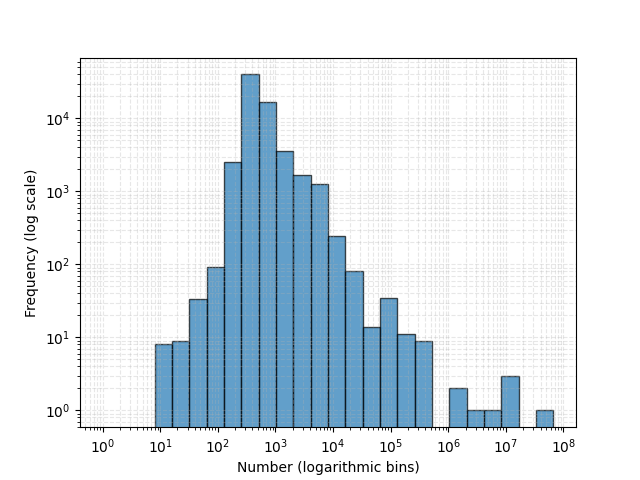
\includegraphics[width=\linewidth]{"./Number of characters, distribution in corpus.png"}}
\caption{Number of characters, distribution in corpus.}
\label{fig}
\end{figure}

\begin{figure}[htbp]
    \centerline{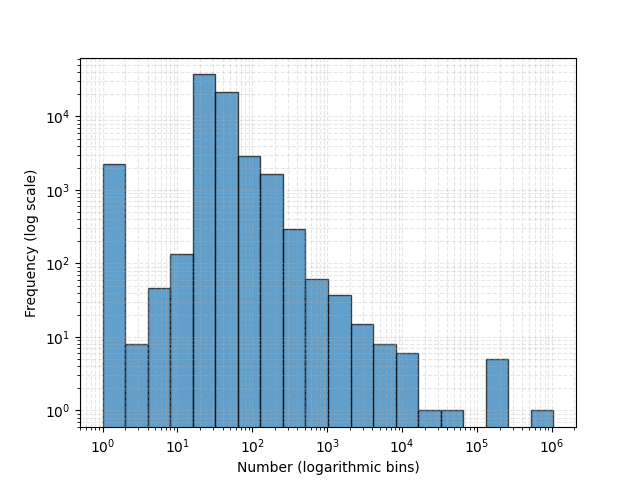
\includegraphics[width=\linewidth]{"./Number of lines, distribution in corpus.png"}}
    \caption{Number of lines, distribution in corpus.}
    \label{fig}
    \end{figure}

    \begin{figure}[htbp]
        \centerline{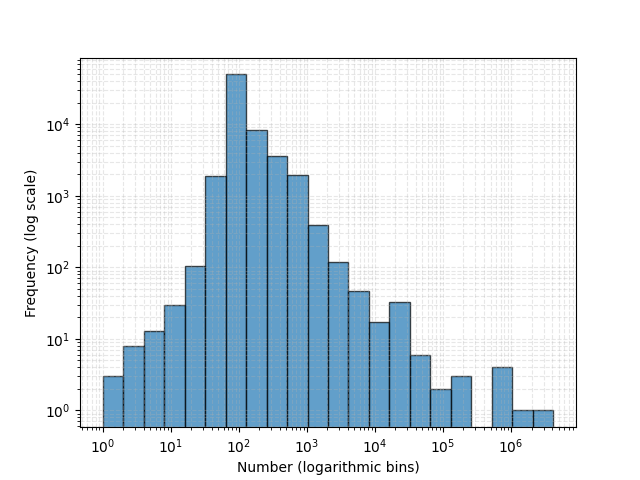
\includegraphics[width=\linewidth]{"./Number of tokens, distribution in corpus.png"}}
        \caption{Number of tokens, distribution in corpus.}
        \label{fig}
        \end{figure}

When examining the number of lines, there seems to be a large number of \verb|.als| files with very few lines (which could be because of a large number of empty or very small models in the corpus).

A similar analysis is carried out for the number of words and sentences in the summaries generated by DeepSeek. The data is split based on the actual summary and the 'think' section, which shows DeepSeek's reasoning.

\begin{figure}[htbp]
    \centerline{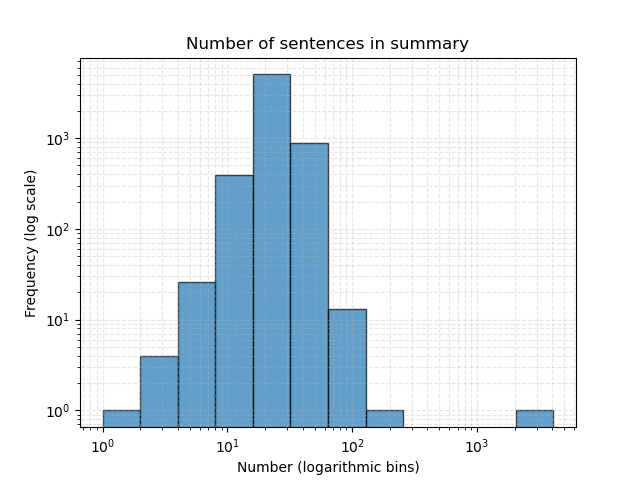
\includegraphics[width=\linewidth]{"./Number of sentences in summary.png"}}
    \caption{Number of sentences in summary.}
    \label{fig}
    \end{figure}

    \begin{figure}[htbp]
        \centerline{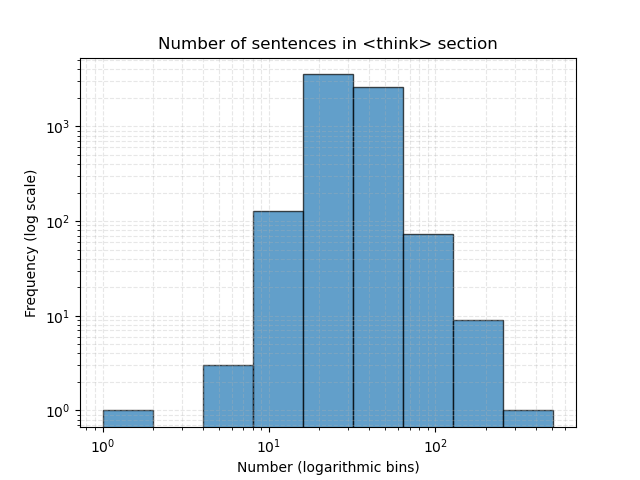
\includegraphics[width=\linewidth]{"./Number of sentences in <think> section.png"}}
        \caption{Number of sentences in 'think' section.}
        \label{fig}
        \end{figure}

        \begin{figure}[htbp]
            \centerline{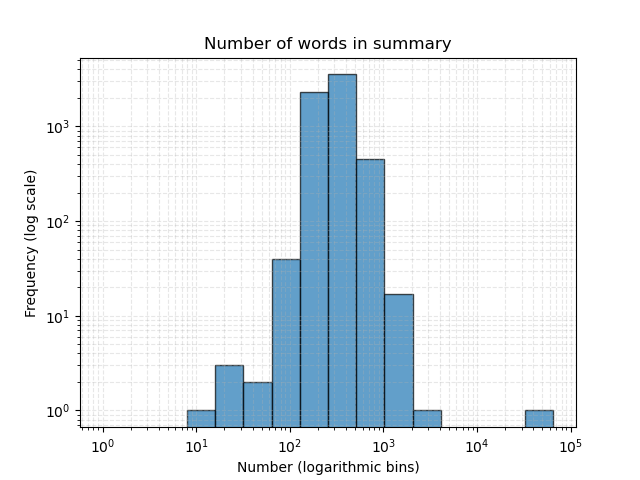
\includegraphics[width=\linewidth]{"./Number of words in summary.png"}}
            \caption{Number of words in summary.}
            \label{fig}
            \end{figure}

            \begin{figure}[htbp]
                \centerline{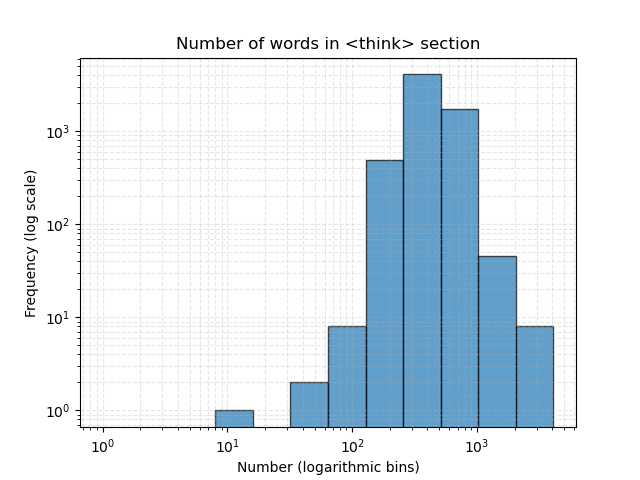
\includegraphics[width=\linewidth]{"./Number of words in <think> section.png"}}
                \caption{Number of words in 'think' section.}
                \label{fig}
                \end{figure}

The relative sharpness of the distribution peaks for the responses, in comparison to the distributions for the original model, show that DeepSeek tends to have a fairly limited response window size.

Further investigation of the relationship between the size of the model being summarized and the size of the summary is shown below:

\begin{figure}[htbp]
    \centerline{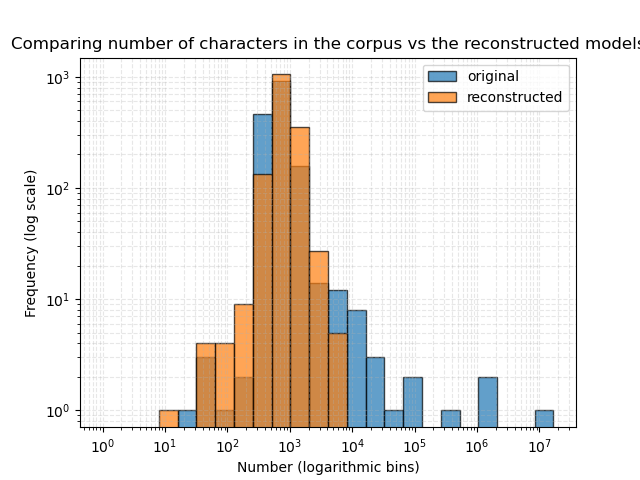
\includegraphics[width=\linewidth]{"./Comparing number of characters in the corpus vs the reconstructed models.png"}}
    \caption{Comparing number of characters in the corpus vs the reconstructed models.}
    \label{fig}
    \end{figure}
    
    
    \begin{figure}[htbp]
    \centerline{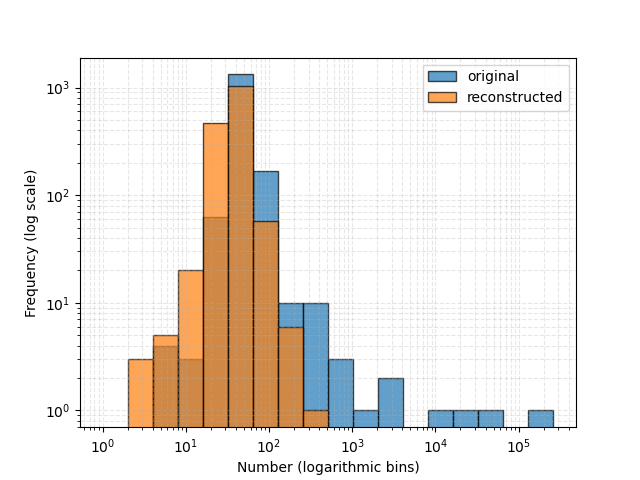
\includegraphics[width=\linewidth]{"./Comparing number of lines in the corpus vs the reconstructed models.png"}}
    \caption{Comparing number of lines in the corpus vs the reconstructed models.}
    \label{fig}
    \end{figure}
    
    
    \begin{figure}[htbp]
    \centerline{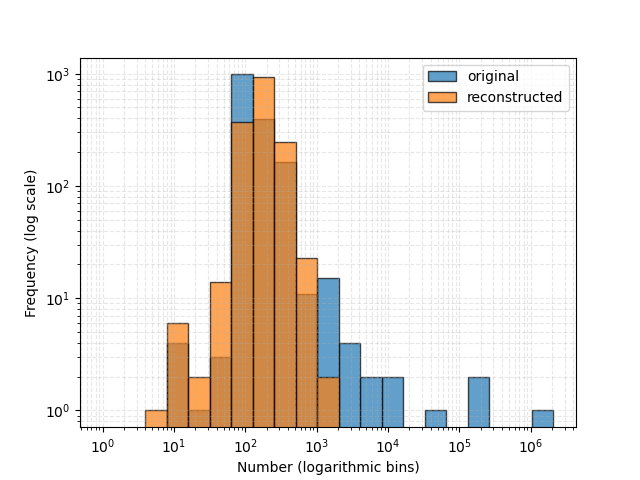
\includegraphics[width=\linewidth]{"./Comparing number of tokens in the corpus vs the reconstructed models.png"}}
    \caption{Comparing number of tokens in the corpus vs the reconstructed models.}
    \label{fig}
    \end{figure}
    

    From the data, it is clear that the LLM is capable of producing models whose length is at or below the mode for the dataset. However, for large models, the reconstructions produced by the LLM rarely reach a similar length. This suggests that the best use of AI involves the creation of small modular Alloy code, rather than large monoliths.

    The difference in distributions at the left tail indicates that the LLM is biased towards generating smaller models than the ones in the corpus. This suggests that in the process of summarization and reconstruction, there is either a decrease in verbosity, or a loss of detail and complexity.
    
    When the relation between the sizes of the original model, the reconstruction and the summary is explored in further detail, the following becomes apparent:

    \begin{figure}[htbp]
        \centerline{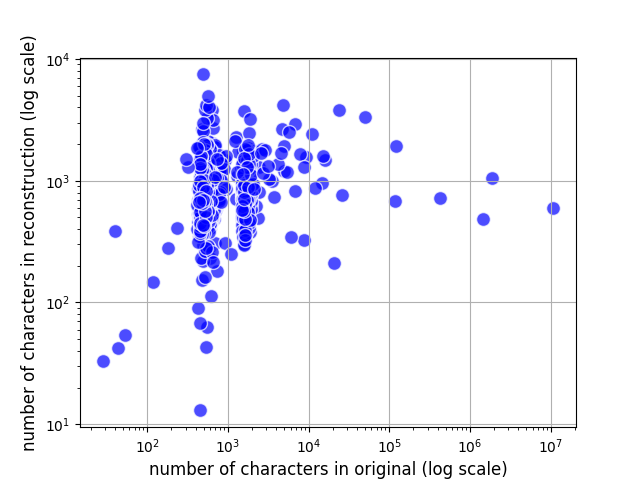
\includegraphics[width=\linewidth]{"./correlation between size of original and reconstructed model.png"}}
        \caption{correlation between size of original and reconstructed model.}
        \label{fig}
        \end{figure}
        
        
        \begin{figure}[htbp]
        \centerline{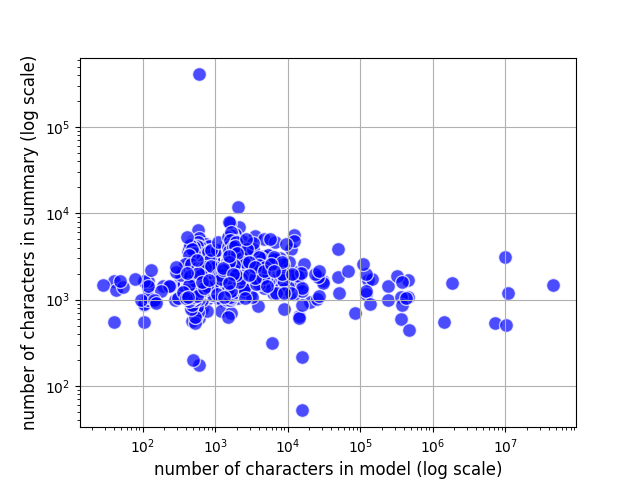
\includegraphics[width=\linewidth]{"./correlation between size of model and LLM-generated summary.png"}}
        \caption{correlation between size of model and LLM-generated summary.}
        \label{fig}
        \end{figure}

        
\begin{itemize}
\item The reconstructed model shows a strong positive correlation upto models of around 1000 lines, after which the size of the reconstructed model plateaus out. This strongly suggests that the LLM tends to recreates models of a similar size as the original, provided it is not hampered by the response window.
\item There is no correlation between the length of the summary and the length of the model being summarized, possibly because the LLM uses all the available response length to explain the model. In case of simple models, the explanation could be more verbose, expanding to fill up the response window.
\end{itemize}

\subsection{Analysis of the Comments}

For languages which are designed to be easily readable, the best coding standards recommend self-commented code whose purpose is evident upon reading (for instance, using practices like descriptive variable names). In case the language's syntax is highly specialized or otherwise difficult to read for the layperson, a liberal policy is recommended for writing comments (since the difficulties cuased by the presence of an unnecessary comment is much less than the absence of a necessary comment).

In general, we expect the corpus to have fewer comments than would be seen in typical production Alloy code in a professional environment, since the corpus includes Alloy code written as part of assignments and small personal projects. When the commenting habits are compared between the corpus and the reconstructed code:

\begin{figure}[htbp]
    \centerline{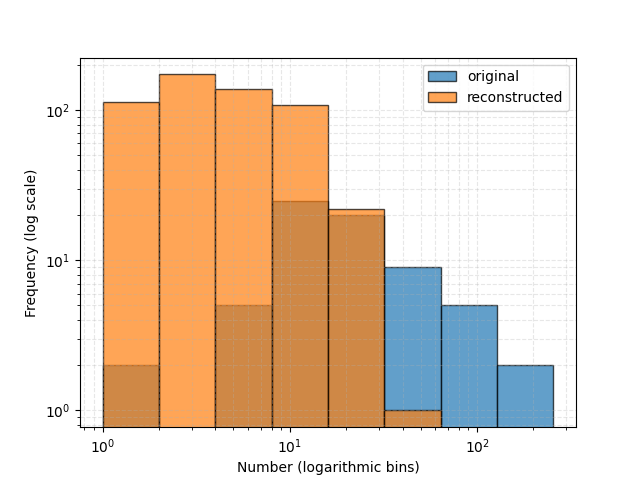
\includegraphics[width=\linewidth]{"./Comparing number of comments in the corpus vs the reconstructed models.png"}}
    \caption{Comparing number of comments in the corpus vs the reconstructed models.}
    \label{fig}
    \end{figure}
    
    
    \begin{figure}[htbp]
    \centerline{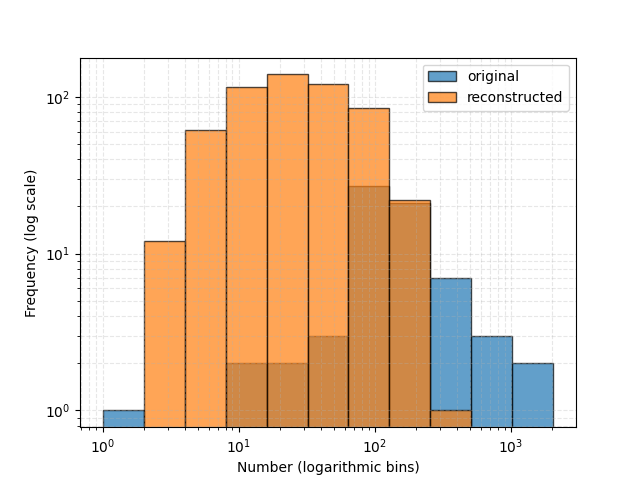
\includegraphics[width=\linewidth]{"./Comparing total number of words in the comments in the corpus vs the reconstructed models.png"}}
    \caption{Comparing total number of words in the comments in the corpus vs the reconstructed models.}
    \label{fig}
    \end{figure}

The key conclusions are:
\begin{itemize}
    \item LLMs tend to comment less when reconstructing a model from a summary, in comparison to the original models.
    \item The comments written by LLMs tend to be shorter than the comments in the original model, possibly because the explanation of each element is presented in a separate section outside the code.
\end{itemize}

The commenting behaviour of LLMs could be amended via amending the prompt to include phrases such as "Explain the code in comments, not in a separate section". LLMs which can reliably do this present a significant advantage to the user, who need not keep switching between the code and the explanation when reading the reconstructed model.

\subsection{Analysis of Signatures}

Alloy models describe relations between atoms, whose types are described by signatures. Inheritance is applied to signatures using the \verb|extends| keyword. For instance, \verb|Man extends Person| and \verb|Woman extends Person| in the earlier example show inheritance, where \verb|Man| and \verb|Woman| are subtypes of \verb|Person|.

\begin{figure}[htbp]
    \centerline{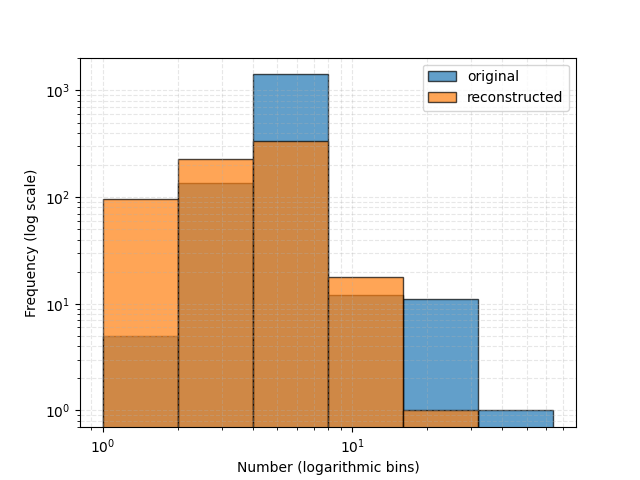
\includegraphics[width=\linewidth]{"./Comparing number of signatures in the corpus vs the reconstructed models.png"}}
    \caption{Comparing number of signatures in the corpus vs the reconstructed models.}
    \label{fig}
    \end{figure}
    
    
    \begin{figure}[htbp]
    \centerline{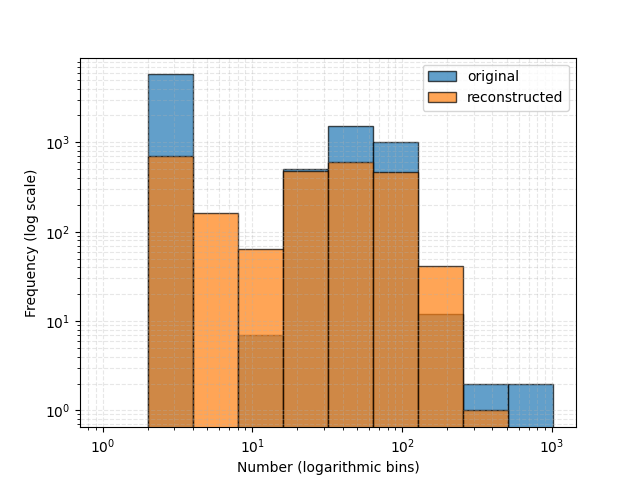
\includegraphics[width=\linewidth]{"./Comparing size of the signature bodies in the corpus vs the reconstructed models.png"}}
    \caption{Comparing size of the signature bodies in the corpus vs the reconstructed models.}
    \label{fig}
    \end{figure}

    When comparing the signatures generated by the LLM with the original corpus:

    The LLM tends to create models with under 10 signatures. This suggests that a low accuracy for the reconstruction of large models, since a reduction in the number of signatures tends to correspond to a reduction in the model's complexity. Poorly designed signature schema could be simplified by merging signatures and eliminating unnecessary abstraction (for instance, \verb|Person| can be eliminated by duplicating its code in both \verb|Man| and \verb|Woman|, reducing the total number of signatures by 1), but such reductions often result in an increase in the sizes of the signatures thus produced, which is not the case as seen in the comparison of sizes, which reveals that the LLM is slightly biased towards producing signatures with smaller sizes.
    
    This suggests that creating multiple \verb|.als| files with a small number of small signatures will result in a better model, which is in line with generally recommended coding practices.

    \begin{figure}[htbp]
        \centerline{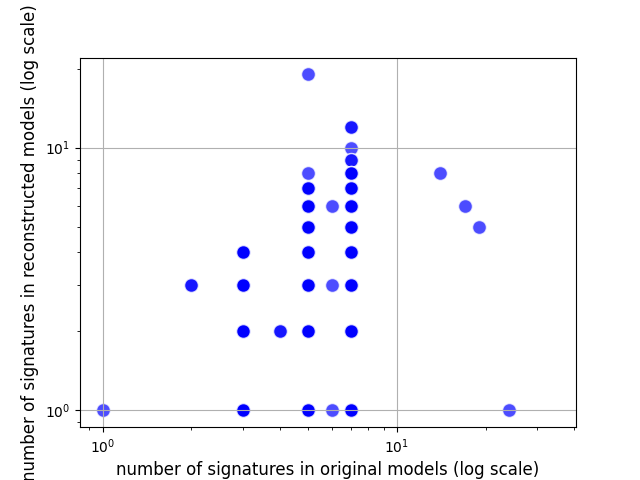
\includegraphics[width=\linewidth]{"./Correlation between number of signatures in the original and reconstructed models.png"}}
        \caption{Correlation between number of signatures in the original and reconstructed models.}
        \label{fig}
        \end{figure}

        This shows that the reconstructed models tends to have a number of signatures less than or equal to the number of signatures in the original model, with a quick drop-off for models having more than 10 signatures, which supports the conclusions drawn from the earlier results.

        Similar analyses, when performed for other elements like facts, preds, asserts and funs, do not produce enough data to draw any strong conclusions. The distributions are included in the appendix.

\subsection{Analysis of Signature Inheritance}

In general, inheritance can be represented via a directed acyclic graph \cite{jackson-reference}, where each node corresponds to a single signature. Signatures are categorized as follows:

\begin{itemize}
    \item type signatures (declared using the \verb|extends| keyword)
    \item subset signatures (declared using the \verb|in| keyword)
\end{itemize}

    Due to additional constraints imposed on type signatures in Alloy, the graph associated with the relations between them forms a forest-like structure, one with a set of rooted trees \cite{jackson-reference}
    in the top-level types.
    
    While determining isomorphism for arbitrary graphs is a hard problem \cite{graph-isomorphism}, determining isomorphism for sets of rooted trees is simple \cite{AHU}.

    \newcommand{\FUNCTION}[2]{\STATE \textbf{function} #1(#2)}
    \newcommand{\ENDFUNCTION}{\STATE \textbf{end function}}

    \begin{center}
        \textbf{Algorithm:} Binary encoding
        \end{center}
        \begin{algorithmic}[1]  % [1] enables line numbers
        \REQUIRE $root$ points to the root node of tree
        \ENSURE $s$ is the binary encoding of $root$
        \FUNCTION{encode}{$root$}
        \IF{$root = nullptr$}
            \RETURN $\varepsilon$
        \ENDIF 
        \STATE $c \gets [encode(c) : c \in root.children]$
        \STATE $s \gets ``0''$
        \STATE Sort $c$ lexicographically
        \FOR{$i \gets 1$ \TO $c.length$}
        \STATE $s \gets s \cdot c[i]$
        \ENDFOR
        \STATE $s \gets s \cdot ``1''$
        \RETURN $s$
        \ENDFUNCTION
        \end{algorithmic}

The given algorithm produces a unique binary string for every rooted tree. For a forest of trees, a new tree is constructed where each top-level node in the forest is a child of a ultimate root node, to which this algorithm is then applied.

\begin{center}
    \textbf{Algorithm:} Tree decoding
    \end{center}
    \begin{algorithmic}[1]  % [1] enables line numbers
    \ENSURE $s$ is the binary encoding of a tree
    \REQUIRE $root$ points to the root node of decoded tree
    \FUNCTION{decode}{$s$}
    \STATE $root \gets nullptr$
    \FOR{$i \gets 1$ \TO $s.length$}
        \STATE $n \gets s[i]$
        \IF{$n = ``0''$}
        \STATE $c \gets Node()$
        \IF{$root \neq nullptr$}
            \STATE $root.children \gets root.children::c$
        \ENDIF
        \STATE $c.parent \gets root$
        \STATE $root \gets c$
        \ELSE
        \STATE $root \gets root.parent$
        \ENDIF
    \ENDFOR
    \RETURN $root$
    \ENDFUNCTION
    \end{algorithmic}

For brevity, a formal proof of correctness of the algorithms is omitted. The existence of a unique encoding and a reversible reconstruction function prove that the encoding is bijective. Applying this algorithm to the graphs associated with type signature inheritance relations, we used it along with a hashtable to enumerate the different inheritance relations in the corpus and identify the relative distributions.


\begin{figure}[htbp]
    \centerline{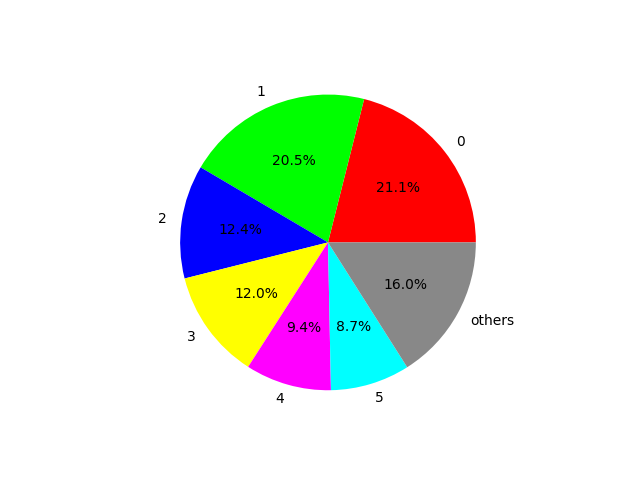
\includegraphics[width=\linewidth]{"./distribution of inheritance hierarchies (original).png"}}
    \caption{distribution of inheritance hierarchies (original).}
    \label{fig}
    \end{figure}

    \begin{figure}[htbp]
        \centerline{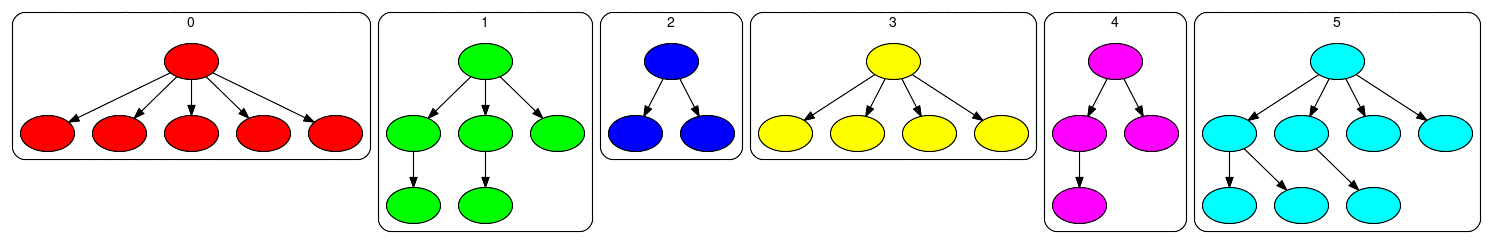
\includegraphics[width=\linewidth]{"./out/original.png"}}
        \caption{Legend: Inheritance Structures (original).}
        \label{fig}
        \end{figure}


The legend shows the graph representations of the inheritance structures, after the introduction of a root node for the forest. The original corpus consists of a large number of models with no inheritance at all (as seen in the graphs with a depth of 1), with a few more complex structures occuring often (as seen in the graphs with a depth greater than 1).
    
    
    \begin{figure}[htbp]
    \centerline{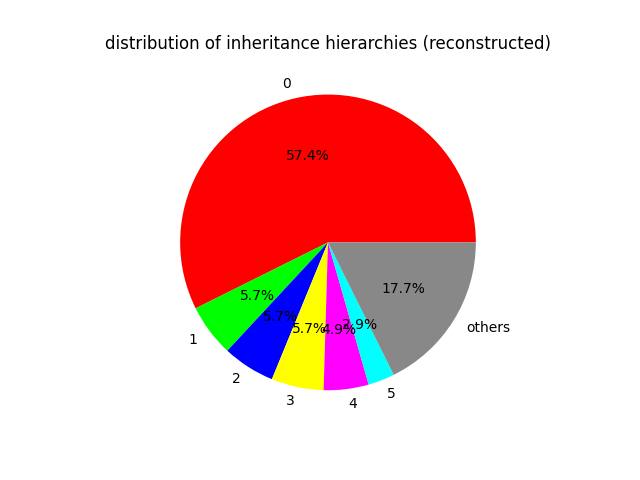
\includegraphics[width=\linewidth]{"./distribution of inheritance hierarchies (reconstructed).png"}}
    \caption{distribution of inheritance hierarchies (reconstructed).}
    \label{fig}
    \end{figure}

    \begin{figure}[htbp]
        \centerline{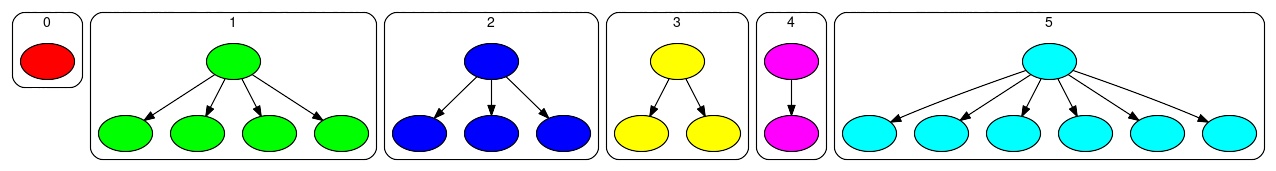
\includegraphics[width=\linewidth]{"./out/reconstructed.png"}}
        \caption{Legend: Inheritance Structures (reconstructed).}
        \label{fig}
        \end{figure}



In comparison, the models generated by the LLM consist mainly of simple inheritance structures, which suggests that the generated code often consists of signatures that do not inherit from other signatures. This could either be due to some inherent bias against inheritance when writing models, or due to the inheritance relations not being captured accurately in the summaries from which the models are reconstructed.

\subsection{Manual Analysis of Summaries}

The analysis of summaries of models was carried out manually after certain automatic filters:

\subsubsection{Length}

To ensure that the models can be understood by a manual reviewer, all models with more than a 100 lines are removed from the dataset. To eliminate trivial models, models with less than 10 lines are removed.

\subsubsection{Duplicate Data}

To remove models which are very similar to each other, the following method was used to measure the degree of similarity between models:

\begin{center}
\textbf{Algorithm:} Model Similarity
\end{center}
\begin{algorithmic}[1]  % [1] enables line numbers
\REQUIRE $s1, s2$ (strings with spaces removed)
\ENSURE $similarity(s1, s2)$
\STATE $N \gets min(s1.length ,s2.length)$
\STATE $ct \gets 0$
\FOR{$i \gets 1$ \TO $N$}
    \IF{$x > 0$}
        \STATE $ct \gets ct + 1$
    \ENDIF
\ENDFOR
\RETURN $ct/N$
\end{algorithmic}
    
For every pair of models $(m1,m2)$ such that the similarity score exceeds $0.5$, one of the models is removed from the dataset. This process continues until no such pairs remain.

\subsubsection{Language}

Since the manual reviewer is familiar only with English, all models with non-ASCII characters were removed (since Alloy syntax and the English is captured completely by the ASCII character set). This was necessary since the language of the summary generated by the LLM is influenced by the language of the comments and keywords in the model text.

\subsubsection{Composition}

The manual reviewer went through the remaining models and eliminated those which were part of bigger projects, where identifiers not present in the text itself were referenced. This was done since such models rely on contextual information not available to the LLM, making the LLM summaries incomplete.

\begin{figure}[htbp]
\centerline{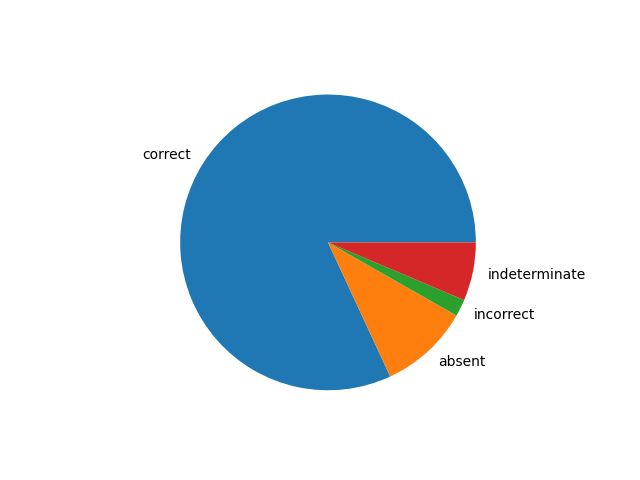
\includegraphics[width=\linewidth]{"./Distribution of ratings from manual analysis.png"}}
\caption{Distribution of ratings from manual analysis.}
\label{fig}
\end{figure}

After these filtration steps, a total of 50 models were chosen for manual review by the reviewer. From the 50 models, a reviewer counts the number of elements in each model (defined as either a \verb|sig|, \verb|fact|, \verb|assert|, \verb|pred| or a \verb|fun|), and the number of elements correctly described in the summary.

\section{Limitations}



\subsection{Selection Bias}

Manual analysis of summaries is carried out only for models which are easy to read. This biases it towards models of around 100 lines, written using English identifiers (which is the language the authors are familiar with).

Large models are left out of the manual analysis. Since the automatic analyses strongly suggest that the performance of the LLM is dependent on the size of the model, the results of the manual analysis cannot be extended to apply to large models.

Very short (or empty) models, with no more than 2 signatures, are often captured exactly by the summary, making manual analysis shed no new light on the performance. Furthermore, such models are unlikely to be used in production, so manual analysis does not result in useful conclusions about the application of LLMs in generating models in industrial software engineering.

\subsection{Correctness of models}

Automatic analyses only describe the coding styles of the LLM and compare it to the styles of the original model. It does not say anything about the correctness of the generated models, since it does not compare the ASTs generated by the Alloy Ananlyzer to check for semantic similarity.

The conclusions drawn from automatic analysis are generally superficial, and cannot be used to make strong conclusions about the LLM's overall effectiveness at model reconstruction.

\subsection{Code analysis}

The analysis is performed via an ad-hoc parser created for the purpose of the project, and not the official Alloy Analyzer, since there is a large section of generated code which is almost syntactically correct, from which producing the official AST is impossible without manual editing to fix syntax errors (a costly process). The custom parser imposes looser conditions on syntactic correctness, which allows it to analyse LLM-generated code which is not strictly compliant with Alloy standards.

Furthermore, only static analysis is performed, since dynamic analysis requires that the code be parsed and excuted by the Analyzer. This poses a significant hindrance to drawing conclusions about the correctness of the generated models.

\subsection{Data duplication}

When assignments are uploaded to GitHub (from which the original model is scraped), the models used in the assignments tend to appear several times in the dataset. This was accounted for in manual analysis (via rejecting multiple instances of similar-looking models, for diversity) but is a significant factor in the automatic analyses. One possible mitigation strategy is to use a distance metric between strings to identify groups of models that appear to originate from the same base model, for deduplication of data.

\section{Future work}

A possible avenue for future work could be a comparative study between different LLMs and their abilities to generate Alloy code. This could cover both general purpose LLMs (like GPT-4, Claude, Gemini etc.) and variants of LLMS specifically trained to develop code (like codellama). As LLMs get more powerful at writing code, we would expect to see an increase in the ability to generate valid and useful Alloy code.

Given a set of valid models, a possible extension of this project is to use the ASTs generated by Alloy Analyzer for structural analysis of the generated code. One can go further and perform dynamic code analysis by running the reconstructed models using Alloy Analyzer to see how closely the outputs align with the original models.


\section{Acknowledgment}

\begin{itemize}
    \item Catayst (Online: https://github.com/WatForm/catalyst) was used to scrape Alloy models from GitHub. 
    \item DeepSeek-r1:8b (hosted at HuggingFace) was used as the LLM
    \item The LLM was run on hardware provided by the University of Waterloo, David Cheriton School of Computer Science
\end{itemize}



\begin{thebibliography}{00}
\bibitem{eid} E. Eid and N. A. Day, ``Static Profiling of Alloy Models,'' in IEEE Transactions on Software Engineering, vol. 49, no. 2, pp. 743-759, 1 Feb. 2023 
\bibitem{mora} F. Mora, ``Synthetic Programming Elicitation for Text-to-Code in Very Low-Resource Programming and Formal Languages,'' arXiv:2406.03636
\bibitem{unnamed} Y. Hong, S. Jiang, Y. Fu, S. Khurshid, ``On the Effectiveness of Large Language Models in Writing Alloy Formulas,''
\bibitem{jackson-model} D. Jackson, ``Software Abstractions - Logic, Language and Analysis'', MIT press, Feb 12 2016, pp. 84--85
\bibitem{jackson-reference} D. Jackson, ``Software Abstractions - Logic, Language and Analysis'', MIT press, Feb 12 2016, Appendix B, pp. 253--265
\bibitem{graph-isomorphism} J. Ren, T. Li, ``Graph isomorphism—Characterization and efficient algorithms,'' in High-Confidence Computing, Volume 4, Issue 4, 2024
\bibitem{AHU} F. Ingels, ``Revisiting Tree Isomorphism: An Algorithmic Bric-à-Brac,'' in HAL Open Science, hal-04232137, Feb 13 2024
\bibitem{catalyst} N. Day, R. Yan, E. Eid, ``catalyst'' Online: https://github.com/WatForm/catalyst
\end{thebibliography}


\section{Appendix}


\begin{figure}[htbp]
    \centerline{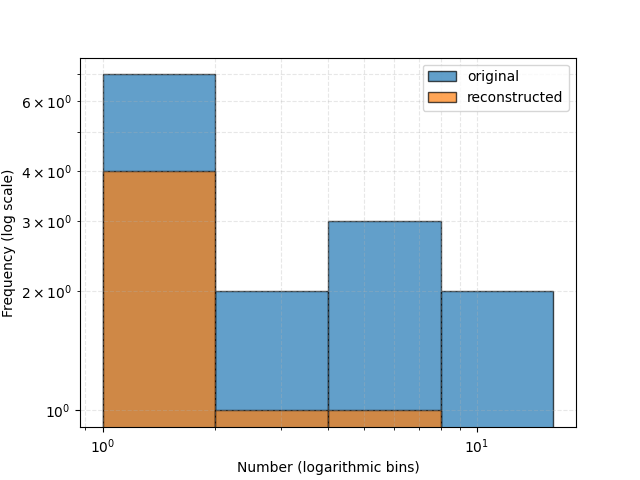
\includegraphics[width=\linewidth]{"./Comparing number of asserts in the corpus vs the reconstructed models.png"}}
    \caption{Comparing number of asserts in the corpus vs the reconstructed models.}
    \label{fig}
    \end{figure}
    
    
    \begin{figure}[htbp]
    \centerline{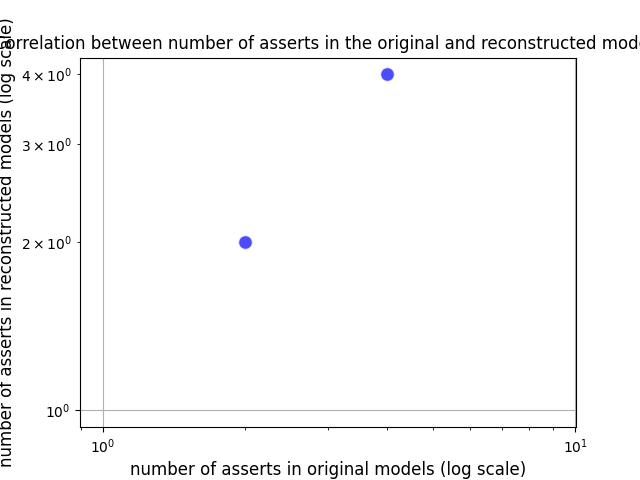
\includegraphics[width=\linewidth]{"./Correlation between number of asserts in the original and reconstructed models.png"}}
    \caption{Correlation between number of asserts in the original and reconstructed models.}
    \label{fig}
    \end{figure}
    
    
    \begin{figure}[htbp]
    \centerline{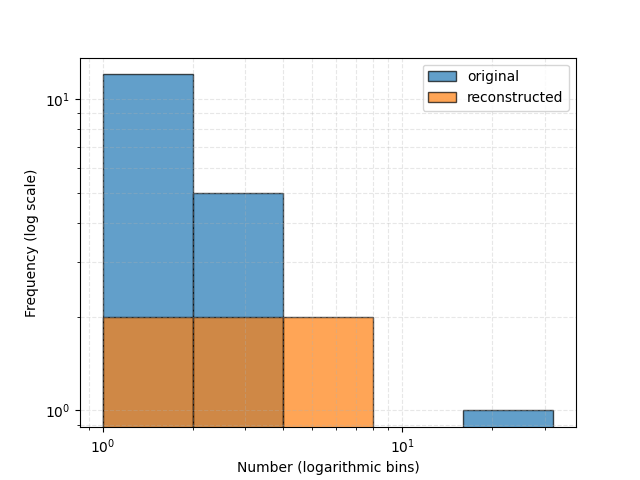
\includegraphics[width=\linewidth]{"./Comparing number of facts in the corpus vs the reconstructed models.png"}}
    \caption{Comparing number of facts in the corpus vs the reconstructed models.}
    \label{fig}
    \end{figure}
    
    
    \begin{figure}[htbp]
    \centerline{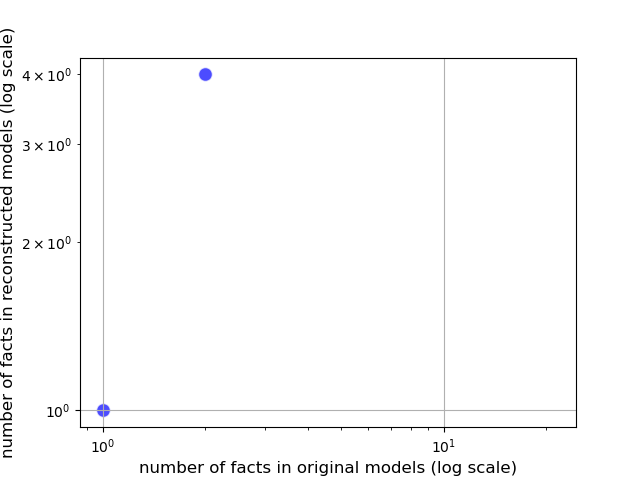
\includegraphics[width=\linewidth]{"./Correlation between number of facts in the original and reconstructed models.png"}}
    \caption{Correlation between number of facts in the original and reconstructed models.}
    \label{fig}
    \end{figure}
    
    
    \begin{figure}[htbp]
    \centerline{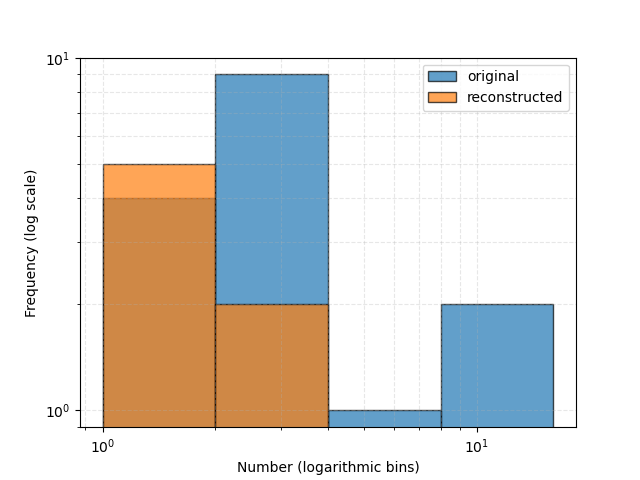
\includegraphics[width=\linewidth]{"./Comparing number of funs in the corpus vs the reconstructed models.png"}}
    \caption{Comparing number of funs in the corpus vs the reconstructed models.}
    \label{fig}
    \end{figure}
    
    
    \begin{figure}[htbp]
    \centerline{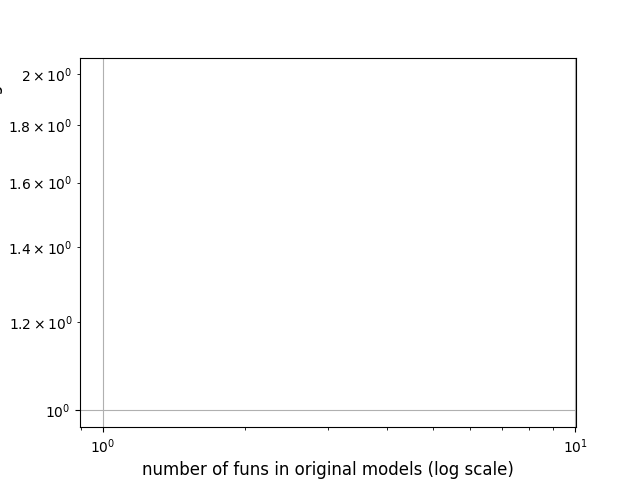
\includegraphics[width=\linewidth]{"./Correlation between number of funs in the original and reconstructed models.png"}}
    \caption{Correlation between number of funs in the original and reconstructed models.}
    \label{fig}
    \end{figure}
    
    
    \begin{figure}[htbp]
    \centerline{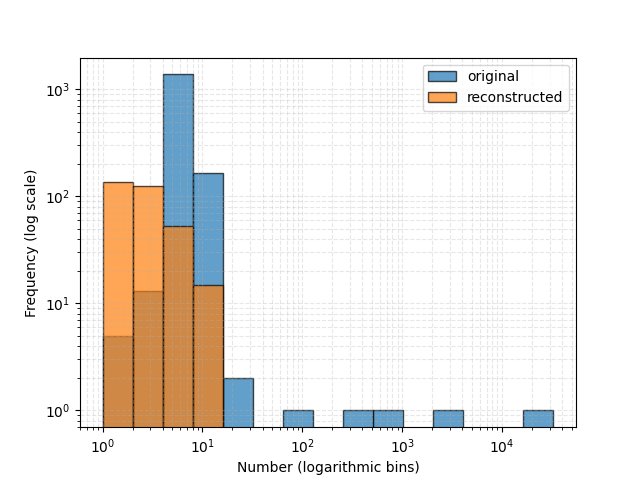
\includegraphics[width=\linewidth]{"./Comparing number of preds in the corpus vs the reconstructed models.png"}}
    \caption{Comparing number of preds in the corpus vs the reconstructed models.}
    \label{fig}
    \end{figure}
    
    
    \begin{figure}[htbp]
    \centerline{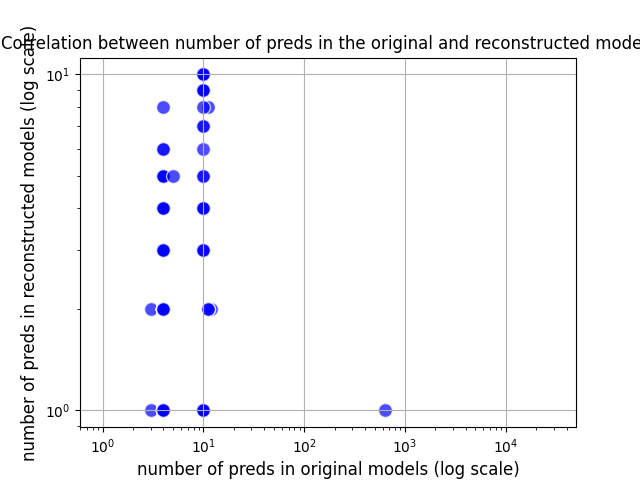
\includegraphics[width=\linewidth]{"./Correlation between number of preds in the original and reconstructed models.png"}}
    \caption{Correlation between number of preds in the original and reconstructed models.}
    \label{fig}
    \end{figure}




\end{document}
